\section{Introducción}

Este proyecto hace referencia a la función de producción de Cobb-Douglas, siendo este publicado en \cite{Douglas1976} 1928 por \citeauthor{Douglas1976}, quienes realizaron un estudio en el que se modeló el crecimiento de la economía estadounidense. Para este proyecto se desarrollará una aplicación con una base de datos como un caso particular, pero previo a su aplicación, se realizará una posible forma de cómo Charles Cobb y Paul Douglas llegaron a la formulación algebraica de la función. Al finalizar, se comparará la solución exacta de la ecuación con la obtenida por el método de mínimos cuadrados.

\subsection{Función de producción de Cobb-Douglas}

Para el análisis matemático de la función, es necesario describir los factores involucrados en el modelo.

\subsection{Función de producción}

Es la relación entre las cantidades máximas de productos que una empresa puede fabricar mediante el uso de diversas cantidades de insumos. Las múltiples funciones de producción están representadas por la combinación de factores de insumo (tecnología, capital, trabajo entre otros). Una función de producción se expresa como la ecuación~\eqref{eq:production} siguiente:
\begin{equation}\label{eq:production}
P=f(K,L,I)
\end{equation}
donde:
\begin{itemize}
	\item $P$ es la cantidad de producción.
	\item $K,L,I$ son los insumos.
\end{itemize}

\section{El proyecto}

En esta sección explicaré los detalles de mi proyecto y su visión. Espero que esta estructura se mejore considerablemente bajo la guía de mi mentor.

\subsection{Cobb-Douglas y la función de producción ACMS}

Partiendo de la función Cobb-Douglas
\begin{equation}%\label{eq:1}
Y = bL^{k}C^{1-k},
\end{equation}
donde:
\begin{itemize}
	\item $b$ representa el factor total de productividad,
	\item $Y$ la producción total,
	\item $L$ el trabajo,
	\item $C$ el capital.
\end{itemize}
Esta función fue generalizada siendo expresada de la manera siguiente:
\begin{equation}%\label{eq:2}
f = \gamma{x}_{1}^{\alpha_{1}}\cdots x_{n}^{\alpha_{n}},
\end{equation}
donde $\gamma$ es una constante positiva y $\alpha_{1},\ldots,\alpha_{n}$ son constantes no cero.

Se dice que una función de producción $f$ es $d$--homogénea o homogénea de degradación $d$, si:
\begin{equation}%\label{eq:3}
f\left(tx_{1},\ldots,tx_{n}\right) = t^{d}f\left(x_{1},\ldots,x_{n}\right),
\end{equation}
Se mantiene para cada $t\in\mathbb{R}$ en la función previamente definida.

Una función \emph{homogénea de degradación uno} es llamado como \emph{linealmente homogéneo}.

Si $d>1$, la función homogénea mostrará un crecimiento a escala, caso contrario cuando $d<1$ mostrará un decrecimiento a escala.

Arrow, Chenery, Minhas y Solow(ACMS) introdujeron una función de producción de dos factores:
\begin{equation}%\label{eq:4}
Q=F\cdot(aK^r + (1-a)L^r)^{1/r},
\end{equation}
donde:
\begin{itemize}
	\item $Q$ representa el resultado,
	\item $F$ el factor de producción,
	\item $a$ el parámetro compartido,
	\item $k,L$ los factores de producción primario,
	\item $r=\left(s-1\right)/s$ , $s=1/\left(1-r\right)$ como la substitución de elasticidad.
\end{itemize}

La función de producción generalizada de ACMS se define:
\begin{equation}\label{eq:5}
f\left(x\right) = \gamma\sum_{i=1}^{n} ({{a}_{i}^{p}x_{i}^{p}})^{d/p},x=\left(x_{1},\ldots,x_{n}\right)\in D\subset\mathbb{R}_{+}^{n},
\end{equation}
con $a_{1},\ldots,a_{n},\gamma,p\neq0$, donde $d$ es la degradación de homogeneidad.

Cabe resaltar que la \emph{función de producción homotética} tiene la siguiente expresión como una función de producción:
\begin{equation}\label{eq:6}
f(x) = F\left(h(x_1,\ldots,x_n\right),
\end{equation}
donde F es una función estrictamente creciente y $h\left(x_1,\ldots,x_n\right)$ es una función homogénea de cualquier degradación d. La \emph{función de producción homotética} de la forma:
\begin{equation}\label{eq:7}
f\left(x\right) = \gamma\sum_{i=1}^{n} ({{a}_{i}^{p}x_{i}^{p}})^{d/p},\quad(\text{resp.},\quad f(x)=F(x_{1}^{\alpha_1}\cdots x_{n}^{\alpha_n}),
\end{equation}
es llamada \emph{función de producción ACMS generalizada homotética}.

\subsection{Breve descripción}

Si $f$ es una función de dos variables, a menudo dejamos que una letra como $z$ denote el valor de $f$ en el punto $\left(x,y\right)$, así $z=f\left(x,y\right)$. Entonces llamaremos a $x$ e $y$ las \emph{variables independientes}, o los \emph{argumentos} de $f$, mientras que $z$ es llamada la \emph{variable independiente}, porque el valor $z$, en general, depende de los valores $x$ e $y$. El dominio de la función $f$ es entonces el conjunto de todos los posibles pares de variables independientes, mientras que su \emph{rango} es el conjunto de valores correspondientes de la variable dependientes. En economía, $x$ e $y$ son llamadas las variables \emph{exógenas}, mientras que $z$ es la variable \emph{endógena}.

Una función de dos variables que aparecen en muchos modelos económicos es
\begin{equation}\label{eq:cobb-douglas}
F\left(x,y\right)=Ax^{a}y^{b}
\end{equation}
donde $A$, $a$ y $b$ son constantes. Usualmente, uno asume que $F$ es definida solo para $x>0$ e $y>0$.

A función de la forma~\eqref{eq:cobb-douglas} es generalmente llamada la \emph{función de Coubb-Douglas}. Se usa con mayor frecuencia para describir ciertos procesos de producción. Entonces $x$ e $y$ son llamados \emph{factores de entrada}, mientras que $F\left(x,y\right)$ es el número de unidades producidas, o la \emph{salida}. En este caso $F$ es llamada la \emph{función de producción}.

%\subsubsection{Defining \pygment{python}{ImageSet} Union for Trigonometric Equation Solver}%\protect||

% TODO: Page 276.
\begin{example}[Elasticidad de sustitución constante]
	Considere la ``elasticidad de sustitución constante'', o la función \textsc{CES}
	\begin{equation}
	F\left(K,L\right)=A\left(aK^{-\rho}+\left(1-a\right)L^{-\rho}\right)^{-1/\rho}
	\end{equation}
	donde $A>0$, $K>0$, $L>0$, $a\in\left(0,1\right)$, y $\rho\neq 0$. Manteniendo $A,K,L$ y $a$ fijos, aplique la regla de L'H\^{o}pital a $z=\ln\left[F\left(K,L\right)/A\right]$  cuando $\rho\to0$ con el fin de mostrar que $F\left(K,L\right)$ converge a la función de Cobb-Douglas $AK^{a}L^{1-a}$.
\end{example}

\begin{proof}[Solución]
	Obtenemos \[ z=\ln{\left(aK^{-\rho}+\left(1-a\right)L^{-\rho}\right)}^{-1/\rho}=-\ln\left(aK^{-\rho}+\left(1-a\right)L^{-\rho}\right)/\rho\to\frac{0}{0}\text{ cuando }\rho\to0. \] Ya que $\left(\mathrm{d}/\mathrm{d}\rho\right)K^{-\rho}=-K^{-\rho}\ln K$ y $\left(\mathrm{d}/\mathrm{d}\rho\right)L^{-\rho}=-L^{-\rho}\ln L$, aplicando la regla de L'H\^{o}pital da
	\begin{align*}
	\lim_{\rho\to0}z
	&=\lim_{\rho\to0}\left[\frac{aK^{-\rho}\ln K + \left(1-a\right)L^{-\rho}\ln L}{aK^{-\rho}+\left(1-a\right)L^{-\rho}}\right]\\
	&=a\ln K+\left(1-a\right)\ln L\\
	&=\ln K^{a}L^{1-a}.
	\end{align*}
	Por lo tanto, $e^{z}\to K^{a}L^{1-a}$. De la definición de $z$, se sigue que $F\left(K,L\right)\to AK^{a}L^{1-a}$ cuando $\rho\to0$.
\end{proof}

%pag. 408-409
\begin{example}[Función de Cobb-Douglas]
	Una función de dos variables que aparece en muchos modelos económicos es
	\begin{equation}\label{eq:cobb}
	F\left(x,y\right)=Ax^{a}y^{b}
	\end{equation}
	donde $A$, $a$ y $b$b son constantes. Usualmente, uno asume que $F$ está definida sola pora $x>0$ e $y>0$.

	Una función $F$ de la forma~\eqref{eq:cobb} es generalmente llamada la \emph{función de Cobb-Douglas}\footnote{La función en~\eqref{eq:cobb} es llamada en honor a los investigadores americanos C.W.Cobb y P.H.Douglas, quien aplicaron esto, con  $a+b=1$, en un articulo científico que aparecio en 1927 en la estimacion de una función de producción. Sin embargo, deberia correctamente ser llamada la ``función de Wicksell'', porque el economista sueco K.Wicksell(1851-1926) introdujo tales funciones de producción antes de 1900.}. Con frecuencia es usada para describir ciertos procesos productivos. Así, $x$ e $y$ son llamados los \emph{factores de entrada}, mientras que $F\left(x,y\right)$ es el número de unidades producidas, o la \emph{salida}. En este caso, $F$ es llamada una \emph{función de producción}.
\end{example}

\begin{example}
	Suponga que $F\left(K,L\right)$ modela la producción de una empresa cuando sus entradas son capital y labor, respectivamente $K$ y $L$. Una curva de nivel por esta función de producción es una curva en el plano $KL$ dado por $F\left(K,L\right)=Y_{o}$, donde $Y_{0}$ es una constante. Esta curva es llamada una \emph{isocuanta}, que significa ``igual cantidad''. Para una función de Cobb-Douglas, $F\left(K,L\right)=AK^{a}L^{b}$, con $a+b<1$ y $A>0$, las figuras~\ref{fig:1} y~\ref{fig:2}, respectivamente, muestra una parte de la gráfica cerca del origen, y tres de las isocuantas.
	
	\begin{figure}[ht!]
		\begin{minipage}[c]{0.4\linewidth}
			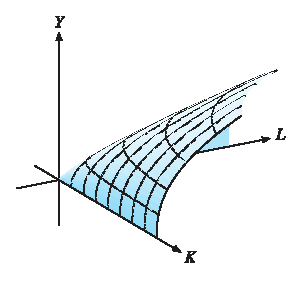
\includegraphics[width=\linewidth]{figure1}\label{fig:1}
			\caption{Gráfica de la función de producción Cobb-Douglas.}
		\end{minipage}
		\hfill
		\begin{minipage}[c]{0.4\linewidth}
			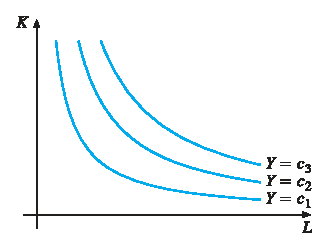
\includegraphics[width=\linewidth]{figure2}\label{fig:2}
			\caption{Isocuantas de la función de producción Cobb-Douglas.}
		\end{minipage}
	\end{figure}
\end{example}
% pag. 428
\begin{example}[Funciones $n$--lineales y $\log$--lineales]
	\leavevmode
	\begin{enumerate}
		\item\label{item:a} La demanda del azúcar en los Estados Unidos durante el período 1929--1936 fue estimado para ser descrito, aproximadamente, por la fórmula \[ x=108.83-6.0294p+0.164w-0.4217t \] donde $x$ es la demanda del azúcar, $p$ es su precio, $w$ es un índice de producción y $t$ es el año (donde $t=0$ corresponde a 1929).
		\item\label{item:b} La siguiente fórmula es una estimación para la demanda de cerveza en el Reino Unido: \[ x=1.058{x}^{0.136}_{1}{x}^{-0.727}_{2}{x}^{0.914}_{3}x^{0.816}_{4}. \]
		Aquí la cantidad demandada, $x$, es una función de cuatro variables: $x_{1}$, el ingreso per cápita, $x_{2}$, el precio de la cerveza, $x_{3}$, índice general de precios de productos básicos y $x_{4}$, la fuerza de la cerveza.
	\end{enumerate}
\end{example}
Las funciones más simples en el ejemplo anterior es la única en la parte~\eqref{item:a}. Las variables $p$, $w$ y $t$ ocurren solo cuando a la primera potencia, y ellas son multiplicadas por constantes, no por cada otra. Tales funciones son llamadas \emph{lineales}. En general
\begin{equation}
f\left(x_{1},x_{2},\ldots,x_{n}\right)=a_{1}x_{1}+a_{2}x_{2}+\cdots+a_{n}x_{n}+b
\end{equation}
donde $a_{1},a_{2},\ldots,a_{n}$ y $b$ son constantes, es una \emph{función lineal} en $n$ variables.

La función en la parte~\eqref{item:b} del ejemplo  es un caso especial de la función general de Cobb-Douglas
\begin{equation}\label{eq:cobbgeneralized}
F\left(x_{1},x_{2},\ldots,x_{3}\right)=A{x}^{a_{1}}_{1}{x}^{a_{2}}_{2}\cdots{x}^{a_{n}}_{n}
\end{equation}
donde $A>0$, $a_{1},\ldots,a_{n}$ son constantes, definidas para $x_{1}>0,x_{2}>0,\ldots x_{n}>0$. Note que al tomar el logaritmo natural a cada lado de~\eqref{eq:cobbgeneralized} resulta
\begin{equation}
\ln F=\ln A+a_{1}\ln x_{1}+a_{2}\ln x_{2}+\cdots+a_{n}\ln x_{n}.
\end{equation}
Esto muestra que la función de Cobb-Douglas es $\log$--lineal, ya que $\ln F$ es una función lineal para $\ln x_{1},\ln x_{2},\ldots,\ln x_{n}$.